\documentclass{beamer}
\usefonttheme[onlymath]{serif}

\usepackage[utf8]{inputenc}
\usepackage[T1]{fontenc}
\usepackage{lmodern}
\usepackage[francais]{babel}

% For table
\usepackage{booktabs} % To thicken table lines
\usepackage{multirow}
\usepackage{amsmath,amssymb,amsfonts}

\graphicspath{{img/}}

\usepackage{graphicx}
\usepackage{textcomp}
\usepackage{xcolor}
\usepackage[group-separator={,}]{siunitx}
\def\BibTeX{{\rm B\kern-.05em{\sc i\kern-.025em b}\kern-.08em
		T\kern-.1667em\lower.7ex\hbox{E}\kern-.125emX}}

\usepackage{booktabs} %top/mid/bottom rule

\definecolor{red}{RGB}{255,0,0}
\definecolor{green}{RGB}{0, 102, 0}
\definecolor{maron}{RGB}{102,51,0}
\definecolor{orange}{RGB}{255,128,0}
\definecolor{blue}{RGB}{0,153,153}

%for footnote
\usepackage{perpage} %the perpage package
\MakePerPage{footnote} %the perpage package command


\mode<presentation> {
	\usetheme{ulaval}
	\setbeamercovered{invisible}
}

\logo{
	
\includegraphics[height=0.65cm, keepaspectratio]{graal.pdf}\hspace{.2cm}\vspace{.85\paperheight}}


\title{Leveraging Subword Embeddings for Multinational Address Parsing\thanks{\url{https://arxiv.org/abs/2006.16152}}}

\author[Yassine et al.]{Marouane Yassine, David Beauchemin, \\ François Laviolette, Luc Lamontagne}
\institute[Université Laval]
{
	Département d'informatique et de génie logiciel, \\
	Université Laval\\
	\medskip
	{\emph{marouane.yassine.1@ulaval.ca, david.beauchemin.5@ulaval.ca, francois.laviolette@ift.ulaval.ca, luc.lamontagne@ift.ulaval.ca}}
}
\date{July 14 2020}

\AtBeginSection[]
{
	\begin{frame}<beamer>
		\frametitle{Agenda}
		\tableofcontents[currentsection]
	\end{frame}
}

\begin{document}
	
	\begin{frame}[label=titre, plain]
		\titlepage
		\begin{center}
			
\includegraphics[height=1cm]{graal}
			
\includegraphics[height=1cm]{UL_P}
		\end{center}
	\end{frame}
	
	\section{Introduction}
	
	\begin{frame}{Introduction}
		What's address parsing?
		\begin{figure}
			\centering
			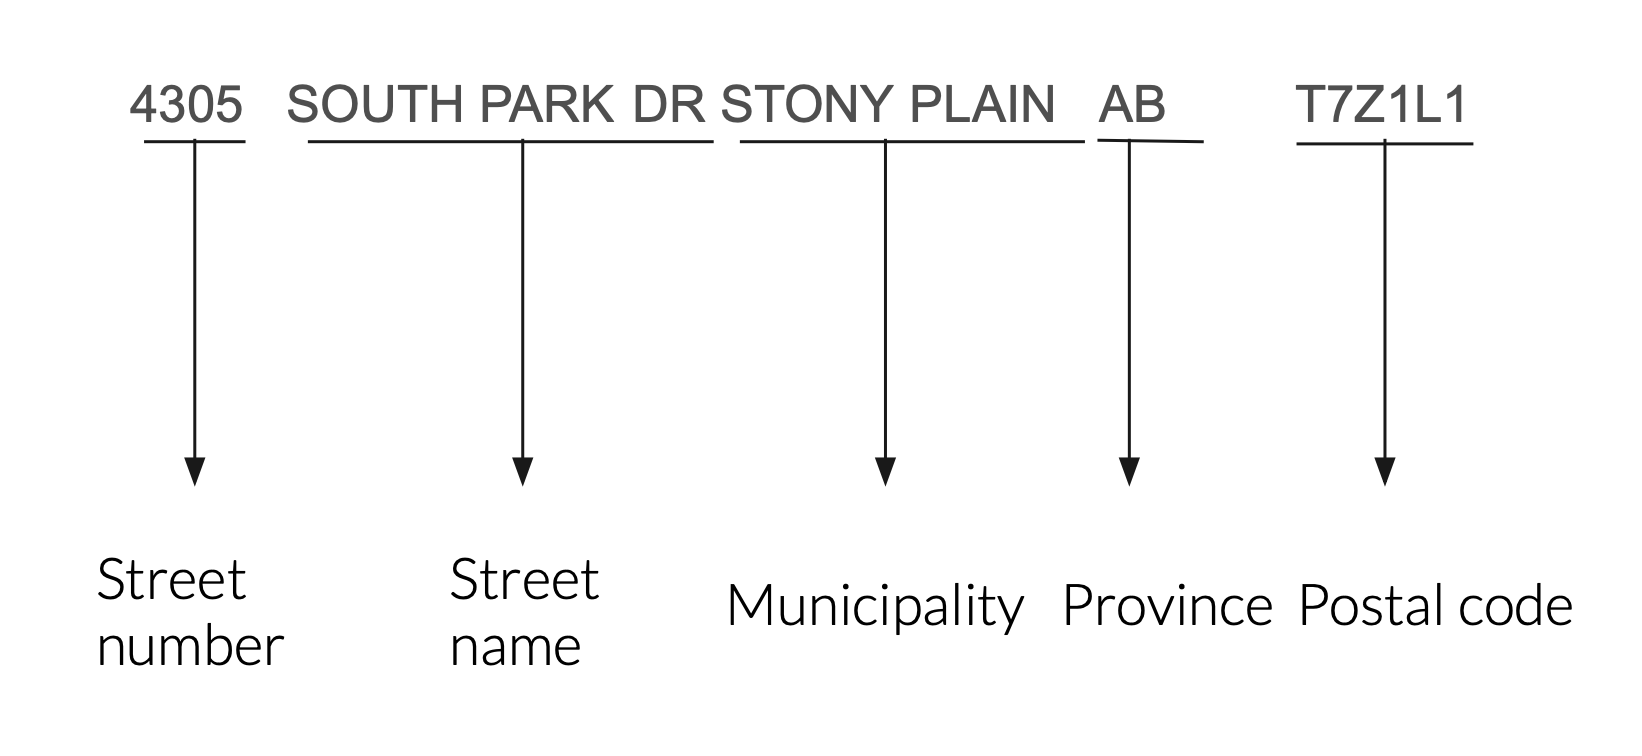
\includegraphics[width=\linewidth]{address_parsing_example.png}
		\end{figure}

		Useful for tasks such as \textit{Record Linkage} and \textit{Geocoding}.
	\end{frame}

	\section{Related Work}
	\subsection{Address parsing for one country}
	\begin{frame}{Related Work - Address Parsing for One Country}
		\begin{itemize}
			\item<1-> Rule based methods
			\item<2-> Probabilistic models
			\begin{itemize}
				\item<2-> Hidden Markov Models (HMM) \cite{hmm-parsing}
				\item<2-> Conditional Random Fields (CRF) \cite{crf-parsing}
			\end{itemize}
			\item<3-> Neural networks
			\begin{itemize}
				\item<3-> Feed-forward Neural Network \cite{feedforward-parsing}
				\item<3-> Recurrent Neural Networks \cite{rnn-parsing}
			\end{itemize}
		\end{itemize}
	\end{frame}

	\subsection{Multinational address parsing}
	\begin{frame}{Related work - Multinational address parsing}
		\textbf{Libpostal} \footnote{\tiny{\url{https://github.com/openvenues/libpostal}}}
		\begin{itemize}
			\item<1-> CRF based model
			\item<2-> Preprocessing and postprocessing
			\item<3-> '\textit{[T]rained on over 1 billion examples in every inhabited country on Earth}' \footnote{\tiny{\url{https://medium.com/@albarrentine/statistical-nlp-on-openstreetmap-part-2-80405b988718}}}
		\end{itemize}

		\vfill

		\uncover<4->{\textbf{No previous neural network approaches for multinational address parsing}}
	\end{frame}

	\section{Subword Embeddings}
	\begin{frame}{Subword Embeddings}
		...
	\end{frame}

	\section{Architecture}
	\begin{frame}{Architecture}
		\begin{figure}[h!]
			\centering
			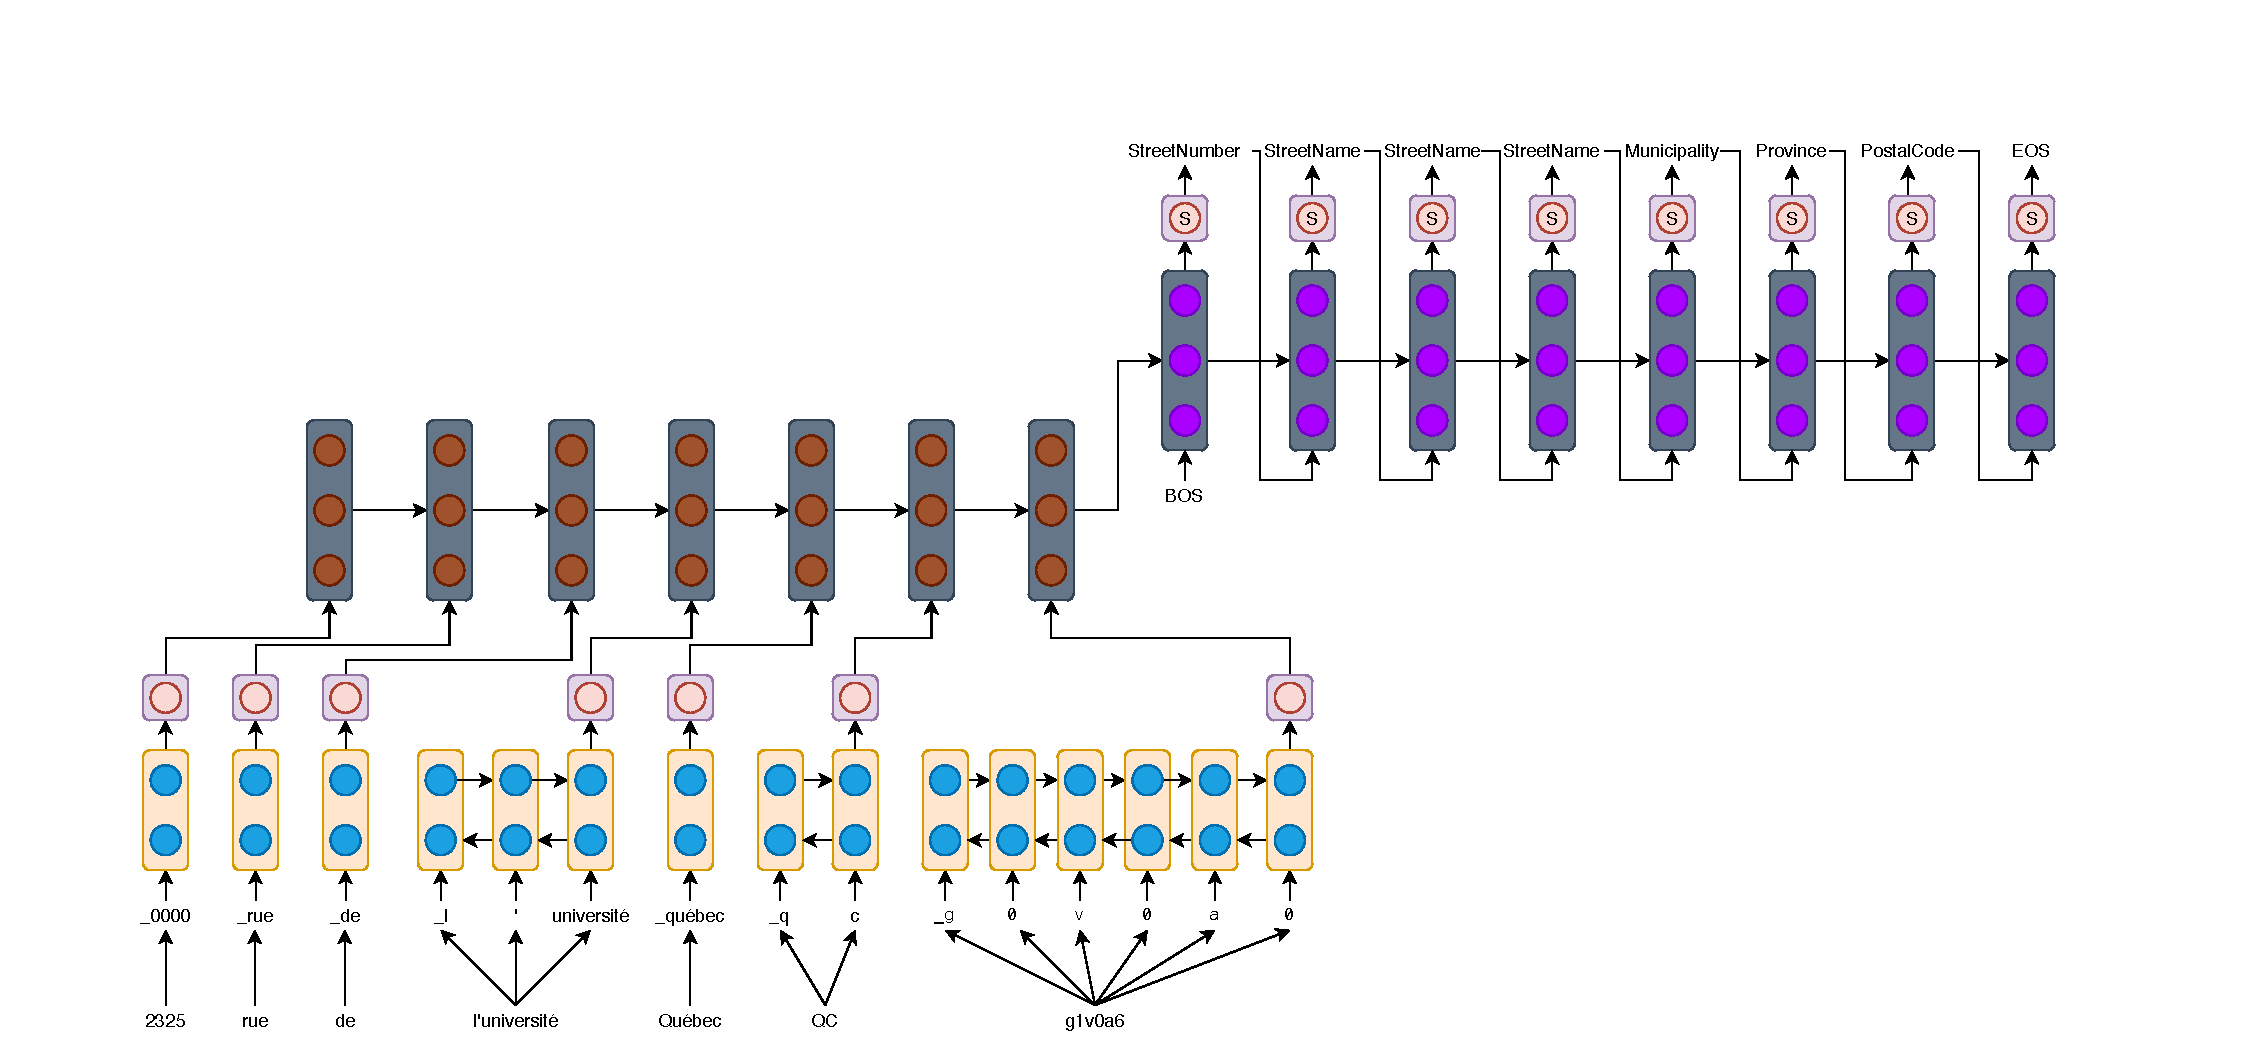
\includegraphics[width=1.1\textwidth,height=\textheight,keepaspectratio]{Network.pdf}
		\end{figure}
	\end{frame}

	\begin{frame}{Embedding Model}
		We compare two pre-trained monolingual embedding.
		\begin{itemize}
			\item<2-> A fixed pre-trained monolingual fastText model (pre-trained on the French language) (\textbf{fastText}).
			\item<3-> A encoding of words using MultiBPEmb and merge the obtained embeddings for each word into one word embedding using a Bidirectional LSTM (Bi-LSTM) (hidden state dimension of $300$). We refer to this embeddings model technique as \textbf{BPEmb}.
		\end{itemize}

		\uncover<4->{We run a comparison of the two methods (\textbf{fastText} and \textbf{BPEmb}) to evaluate which one gives better results in our setting.}
	\end{frame}

	\begin{frame}{Tagging Model}
		We use a Seq2Seq model consisting of
		\begin{itemize}
			\item<2-> a one-layer unidirectional LSTM encoder
			\item<3-> a one-layer unidirectional LSTM decoder
			\item<4-> a fully-connected linear layer with a softmax activation. 
		\end{itemize}
		
		\uncover<5->{Both the encoder's and decoder's hidden states are of dimension $1024$.}
	\end{frame}
	
	\section{Data}
	\begin{frame}{About the Data}
		\begin{itemize}
			\item<1-> Built using the open-source data on which Libpostal's models were trained.
			\item<2-> Contain $61$ countries.
			\item<2-> We used eight tags: StreetNumber, StreetName, Unit, Municipality, Province, PostalCode, Orientation, and GeneralDeliver \footnote{Libpostal used $20$ tags.}.
		\end{itemize}
	\end{frame}	

	\begin{frame}{Examples of Address and Their Patterns}
			We use five different address patterns (one for each color) and another for some countries' using more than a pattern (no color).
			\uncover<2->{\begin{figure}[h!]
				\centering
				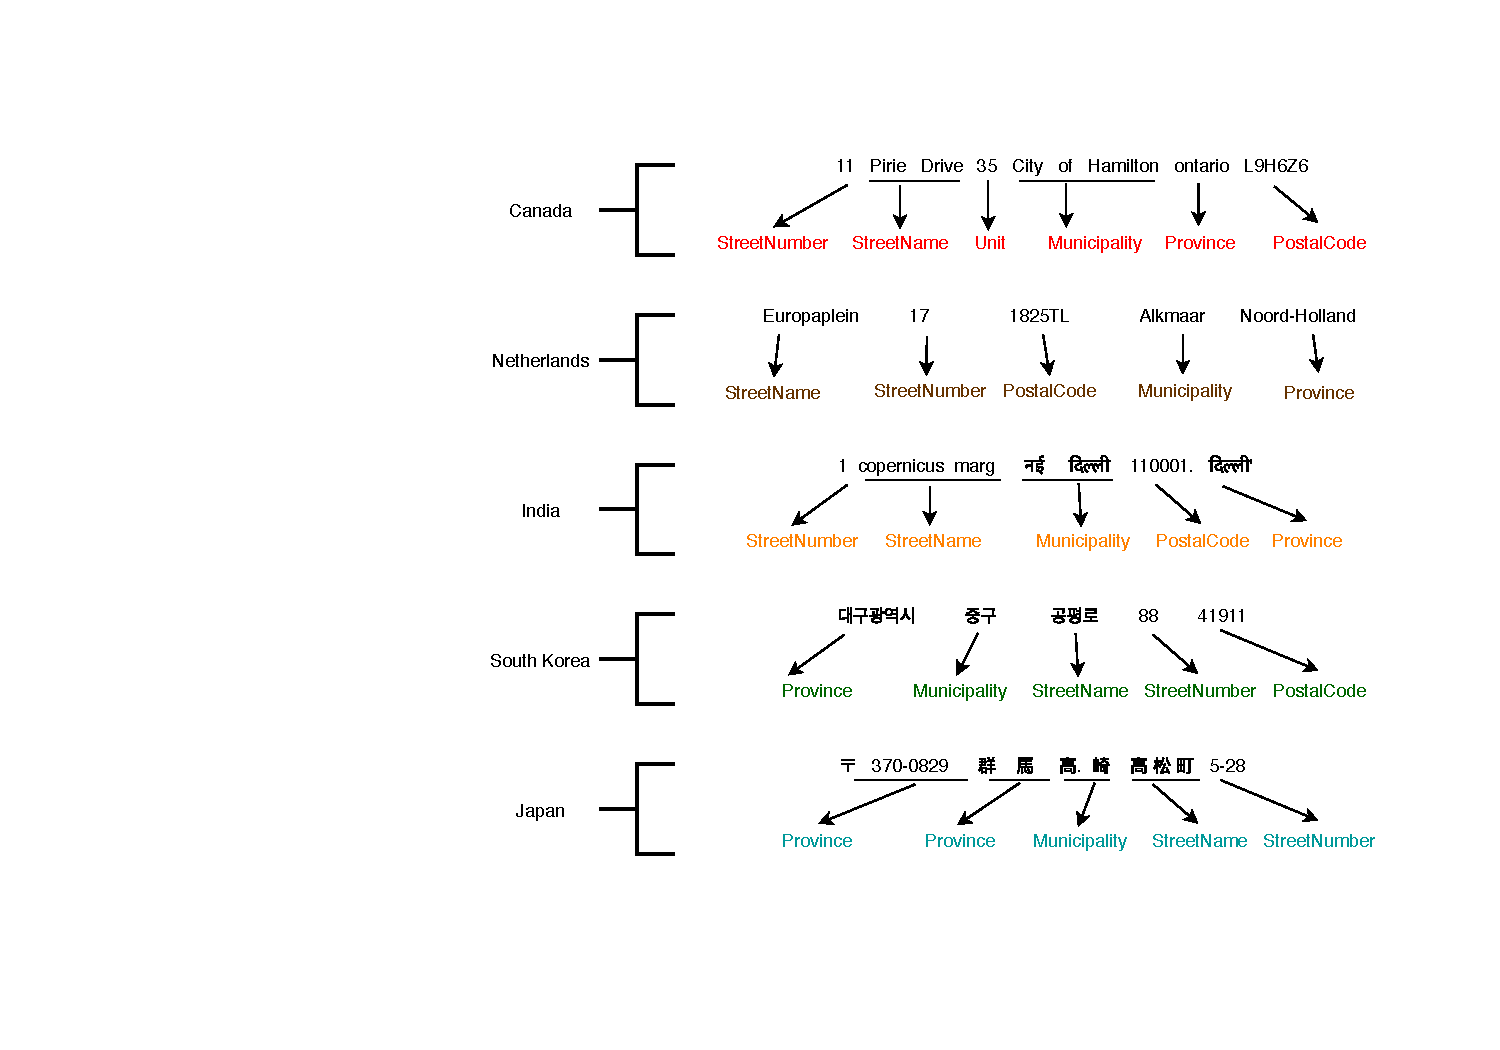
\includegraphics[width=0.8\textwidth,height=0.75\textheight,keepaspectratio]{Samples2.pdf}
			\end{figure}}
	\end{frame}

	\begin{frame}{Training Data and Holdout Test Set}
		$20$ countries are used for multinational training with a sample size of $100,000$ per country. The rest is used as a holdout (table below). \\\bigskip
		
		\resizebox{\textwidth}{!}{%
			\begin{tabular}{cccccccc}
				\toprule
				Country & Number of samples & Country & Number of samples & Country & Number of samples & Country & Number of samples \\ \midrule
				\color{red}United States & \num{8000000} & \color{maron}Germany & \num{1576059} & \color{maron}Poland & \num{459522} &  \color{maron}Czechia & \num{195269} \\ 
				\color{red}Brazil & \num{8000000} & \color{maron}Spain & \num{1395758} & \color{maron}Norway & \num{405649} & \color{maron} Italy & \num{178848} \\ 
				\color{green}South Korea & \num{6048106} & \color{maron}Netherlands & \num{1202173} & \color{maron}Austria & \num{335800} &  \color{maron}France & \num{20050} \\ 
				\color{red}Australia & \num{5428043} & \color{red}Canada & \num{910891} & \color{maron}Finland & \num{280219} &  \color{red}United Kingdom & \num{14338} \\ 
				\color{maron}Mexico & \num{4853349} & \color{maron}Switzerland & \num{474240} & \color{maron}Denmark & \num{199694} &  \color{red}Russia & \num{8115} \\
				\bottomrule
			\end{tabular}%
		}	
	\end{frame}

	\begin{frame}{Zero-Shot Test Set}
		$41$ countries are used for zero-shot transfer evaluation (never seen in training) (table below). \\\bigskip
		
		\resizebox{\textwidth}{!}{%
		    \begin{tabular}{cccccccc}
				\toprule
				Country & Number of samples & Country & Number of samples & Country & Number of samples & Country & Number of samples \\ \midrule
				\color{maron}Belgium & \num{66182} & \color{maron}Slovenia & \num{9773} & \color{maron}Réunion & \num{2514} &  \color{red}Singapore & \num{968} \\ 
				\color{maron}Sweden & \num{32291} & \color{red}Ukraine & \num{9554} & \color{maron}Moldova & \num{2376} &  \color{red}Bangladesh & \num{888} \\ 
				\color{maron}Argentina & \num{27692} & Belarus & \num{7590} & \color{red}Indonesia & \num{2259} &  \color{maron}Paraguay & \num{839} \\ 
				\color{orange}India & \num{26084} & \color{maron}Serbia & \num{6792} & \color{red}Bermuda & \num{2065} &  \color{maron}Cyprus & \num{836} \\ 
				\color{maron}Romania & \num{19420} & \color{maron}Croatia & \num{5671} & \color{maron}Malaysia & \num{2043} &  \color{maron}Bosnia & \num{681} \\ 
				\color{maron}Slovakia & \num{18975} & \color{maron}Greece & \num{4974} & \color{red}South Africa & \num{1388} &  \color{red}Ireland & \num{638} \\ 
				Hungary & \num{17460} & \color{red}New Zealand & \num{4678} & \color{red}Latvia & \num{1325} &  \color{maron}Algeria & \num{601} \\ 
				\color{blue}Japan & \num{14089} & \color{maron}Portugal & \num{4637} & \color{blue}Kazakhstan & \num{1087} &  \color{maron}Colombia & \num{569} \\ 
				\color{red}Venezuela & \num{10696} & \color{maron}Lithuania & \num{3126} & \color{maron}New Caledonia & \num{1036} & Uzbekistan & \num{505} \\ 
				Philippines & \num{10471} & \color{maron}Faroe Islands & \num{2982} & \color{maron}Estonia & \num{1024} &  &  \\ 
				\bottomrule
		\end{tabular}%
		}	
	\end{frame}

	\section{Experiments}
	\begin{frame}{Training Procedure}
		\begin{itemize}
			\item<1-> We trained five times\footnote{With the following seed $\{5, 10, 15, 20, 25\}$} each of our two model (\textbf{fastText} and \textbf{BPEmb}).
			\item<2-> They were trained during $200$ epochs with a batch size of $2048$.
			\item<3-> We used an early stopping with a patience of 15 epochs.
			\item<4-> A starting learning rate at $0.1$ and a learning rate scheduling (factor of $0.1$) after ten epochs without loss decrease. 
			\item<5-> Cross-Entropy loss.
			\item<6-> Stochastic Gradient Descent (SGD) optimizer.
			\item<7-> Teacher forcing \cite{6795228}.
		\end{itemize}
	\end{frame}
	
	
	\begin{frame}{Multinational Evaluation}
		\resizebox{\textwidth}{!}{%
			\begin{tabular}{cccccc}
				\toprule
				Country & \textbf{FastText} & \textbf{BPEmb} & Country & \textbf{FastText} & \textbf{BPEmb}\\
				\midrule
				United States & $\mathbf{99.61 \pm 0.09}$ & $98.55 \pm 2.19$ & Poland & $\mathbf{99.69 \pm 0.07}$ & $99.19 \pm 1.39$\\
				Brazil & $\mathbf{99.40 \pm 0.10}$ & $98.54 \pm 1.68$ & Norway & $\mathbf{99.46 \pm 0.06}$ & $97.98 \pm 1.31$\\
				South Korea & $99.96 \pm 0.01$ & $\mathbf{99.99 \pm 0.02}$ & Austria & $\mathbf{99.28 \pm 0.03}$ & $98.28 \pm 1.56$\\
				Australia & $\mathbf{99.68 \pm 0.05}$ & $99.21 \pm 1.17$ & Finland & $\mathbf{99.77 \pm 0.03}$ & $99.72 \pm 0.30$\\
				Mexico & $\mathbf{99.60 \pm 0.06}$ & $98.55 \pm 2.22$ & Denmark & $\mathbf{99.71 \pm 0.07}$ & $99.20 \pm 1.38$\\
				Germany & $\mathbf{99.77 \pm 0.04}$ & $99.23 \pm 1.30$ & Czechia & $\mathbf{99.57 \pm 0.09}$ & $98.77 \pm 2.22$\\
				Spain & $\mathbf{99.75 \pm 0.05}$ & $98.65 \pm 2.36$ & Italy & $\mathbf{99.73 \pm 0.05}$ & $98.91 \pm 1.76$\\
				Netherlands & $\mathbf{99.61 \pm 0.07}$ & $99.26 \pm 1.23$ & France & $\mathbf{99.66 \pm 0.08}$ & $98.65 \pm 2.00$\\
				Canada & $\mathbf{99.79 \pm 0.05}$ & $99.19 \pm 1.33$ & United Kingdom & $\mathbf{99.61 \pm 0.10}$ & $98.66 \pm 2.11$\\
				Switzerland & $\mathbf{99.53 \pm 0.09}$ & $99.49 \pm 0.53$ & Russia & $\mathbf{99.03 \pm 0.24}$ & $97.52 \pm 4.23$\\
				\bottomrule
			\end{tabular}%
		}
	
	\begin{itemize}
		\item<2-> \textbf{FastText} give the best performance across the board without considering the standard deviation. 
		\item<3-> South Korean results are excellent despite the completely different alphabet.
	\end{itemize}
	\end{frame}

	\begin{frame}{Multinational Evaluation}
		\begin{itemize}
			\item<1-> When using standard deviation, the \textbf{BPEmb} model achieves better results than \textbf{fastText} in most cases. 
			\item<2-> We find that South Korea is the only country where a perfect accuracy ($100~\%$) was achieved using \textbf{BPEmb} ($3$ out of $5$). 
			\item<3-> Randomly reordering $6000$ South Korean address as either the first (red) or the second (brown) address pattern (equally divided between the two), the mean accuracy drops to $28.04\%$.
		\end{itemize}
	\end{frame}

	\begin{frame}{Zero-shot Evaluation}
		\resizebox{\textwidth}{!}{%
		    \begin{tabular}{cccccc}
				\toprule
				Country & \textbf{FastText} & \textbf{BPEmb} & Country & \textbf{FastText} & \textbf{BPEmb}\\
				\midrule
				Belgium & $\mathbf{88.14 \pm 1.04}$ & $87.45 \pm 1.37$ & Faroe Islands & $74.14 \pm 1.83$ & $\mathbf{86.59 \pm 2.21}$\\
				Sweden & $81.59 \pm 4.53$ & $\mathbf{88.30 \pm 2.92}$ & Réunion & $\mathbf{96.80 \pm 0.45}$ & $92.42 \pm 2.38$\\
				Argentina & $\mathbf{86.26 \pm 0.47}$ & $86.00 \pm 4.40$ & Moldova & $\mathbf{90.18 \pm 0.79}$ & $78.11 \pm 16.79$\\
				India & $69.09 \pm 1.74$ & $\mathbf{76.33 \pm 7.77}$ & Indonesia & $64.31 \pm 0.84$ & $\mathbf{69.25 \pm 2.81}$\\
				Romania & $\mathbf{94.49 \pm 1.52}$ & $90.52 \pm 2.35$ & Bermuda & $92.31 \pm 0.60$ & $\mathbf{92.65 \pm 1.84}$\\
				Slovakia & $82.10 \pm 0.98$ & $\mathbf{89.40 \pm 5.09}$ & Malaysia & $78.93 \pm 3.78$ & $\mathbf{92.76 \pm 2.55}$\\
				Hungary & $\mathbf{48.92 \pm 3.59}$ & $24.61 \pm 3.35$ & South Africa & $\mathbf{95.31 \pm 1.68}$ & $92.75 \pm 7.43$\\
				Japan & $\mathbf{41.41 \pm 3.21}$ & $33.34 \pm 3.83$ & Latvia & $\mathbf{93.66 \pm 0.64}$ & $72.46 \pm 5.77$\\
				Iceland & $96.55 \pm 1.20$ & $\mathbf{97.61 \pm 0.98}$ & Kazakhstan & $86.33 \pm 3.06$ & $\mathbf{88.28 \pm 11.32}$\\
				Venezuala & $\mathbf{94.87 \pm 0.53}$ & $89.82 \pm 5.74$ & New Caledonia & $\mathbf{99.48 \pm 0.15}$ & $96.44 \pm 5.64$\\
				Philippines & $77.76 \pm 3.97$ & $\mathbf{78.00 \pm 11.75}$ & Estonia & $\mathbf{87.08 \pm 1.89}$ & $76.18 \pm 1.62$\\
				Slovenia & $95.37 \pm 0.23$ & $\mathbf{96.47 \pm 2.05}$ & Singapore & $\mathbf{86.42 \pm 2.36}$ & $83.23 \pm 6.38$\\
				Ukraine & $\mathbf{92.99 \pm 0.70}$ & $90.86 \pm 2.90$ & Bangladesh & $78.61 \pm 0.43$ & $\mathbf{79.77 \pm 3.65}$\\
				Belarus & $\mathbf{91.08 \pm 3.08}$ & $90.16 \pm 11.89$ & Paraguay & $96.01 \pm 1.23$ & $\mathbf{96.22 \pm 1.78}$\\
				Serbia & $\mathbf{95.31 \pm 0.48}$ & $88.49 \pm 7.05$ & Cyprus & $\mathbf{97.67 \pm 0.34}$ & $92.92 \pm 6.94$\\
				Croatia & $\mathbf{94.59 \pm 2.21}$ & $88.17 \pm 4.58$ & Bosnia & $\mathbf{84.04 \pm 1.47}$ & $80.53 \pm 6.56$\\
				Greece & $\mathbf{81.98 \pm 0.60}$ & $35.30 \pm 13.51$ & Ireland & $\mathbf{87.44 \pm 0.69}$ & $84.93 \pm 2.85$\\
				New Zealand & $94.27 \pm 1.50$ & $\mathbf{97.77 \pm 3.23}$ & Algeria & $\mathbf{85.37 \pm 2.05}$ & $79.66 \pm 11.68$\\
				Portugal & $\mathbf{93.65 \pm 0.46}$ & $90.13 \pm 4.47$ & Colombia & $\mathbf{87.81 \pm 0.92}$ & $87.60 \pm 3.61$\\
				Bulgaria & $\mathbf{91.03 \pm 2.07}$ & $87.44 \pm 11.94$ & Uzbekistan & $\mathbf{86.76 \pm 1.13}$ & $73.75 \pm 3.42$\\
				Lithuania & $\mathbf{87.67 \pm 3.05}$ & $75.67 \pm 2.19$ &  &  & \\
				\bottomrule
			\end{tabular}%
		}	
	\end{frame}

	\begin{frame}{Zero-shot Evaluation}
		\begin{itemize}
			\item<1-> $50~\%$ ($19$ out of $41$) near state-of-the-art performance ($>90~\%$) for \textbf{fastText}. Or $35~\%$ for \textbf{BPEmb}.
			\item<2-> $80~\%$ ($34$ out of $41$) good performance ($>80~\%$) for \textbf{fastText}. Or $65~\%$ for \textbf{BPEmb}.
			\item<3-> The lowest results (below $70\%$) occur for countries where the address pattern and the country official language were not seen in the training data such as India, Hungary, and Japan. 
		\end{itemize}
	\end{frame}

	\begin{frame}{Zero-shot Evaluation}
		For Hungary and Japan, the poorest results of all are mostly due to the address structure (blue), which is the near inverse of the two most present ones (red and brown) (never seen structure and language).
		\newline\bigskip
		
		But, Kazakhstan, which uses the same address pattern as Japan, achieves better results. The main difference being the presence of one of the official language (Kazakh and \textbf{Russian}) in the training dataset. 
		
		\note{Moreover, India achieves almost $20\%$ better results than Hungary and Japan, even if Hindi does not occur in the training dataset. This is probably due to the use of a nearly identical address pattern as the first one (red). The only difference being the inversion of the province and the postal code. It could mean that if no shared language root is present, a shared address structure allows a decent parsing of the address (almost $70\%$).}

	\end{frame}
	
	\section{Conclusion}
	\begin{frame}{Future Work}
		\begin{itemize}
			\item<1-> Attention mechanism \cite{bahdanau2014neural}.
			\item<2-> Domain-adversarial training techniques (e. g. DANN) \cite{ganin2015domainadversarial}.
		\end{itemize}
	\end{frame}
	\begin{frame}{Conclusion}
		\begin{itemize}
			\item<1-> Tackled the multinational address parsing problem with SOTA results.
			\item<2-> Shown that subword embeddings thelp to solve the multilingual aspect of our task.
			\item<3-> We explored the possibility of zero-shot transfer across countries and achieved interesting, but not yet optimal results.
		\end{itemize}		
		\uncover<4->{For more, read the full article \url{https://arxiv.org/abs/2006.16152}}
	\end{frame}

	\begin{frame}{Acknowledgment}
		\begin{itemize}
			\item This research was supported by the Natural Sciences and Engineering Research Council of Canada (IRCPJ 529529-17) and a Canadian insurance company. 
			\item François Laviolette and Luc Lamontagne for their mentorship in this research.
			\item Our colleagues at the GRAAL for their comments and reviews.
		\end{itemize}
	\end{frame}

	\begin{frame}[t, allowframebreaks]
		\frametitle{References}
		\bibliographystyle{apalike}
		\bibliography{bibliography}
	\end{frame}
		
	
\end{document}